% !TEX root = main.tex
\subsubsection*{Event별 Audit 추가 비용}
같은 Event 종류의 Audit off/on을 비교한다. $\Delta C=C_{on}-C_{off}$, $\Delta G=G_{on}-G_{off}$이며 증가율의 분모는 off다.
\begin{center}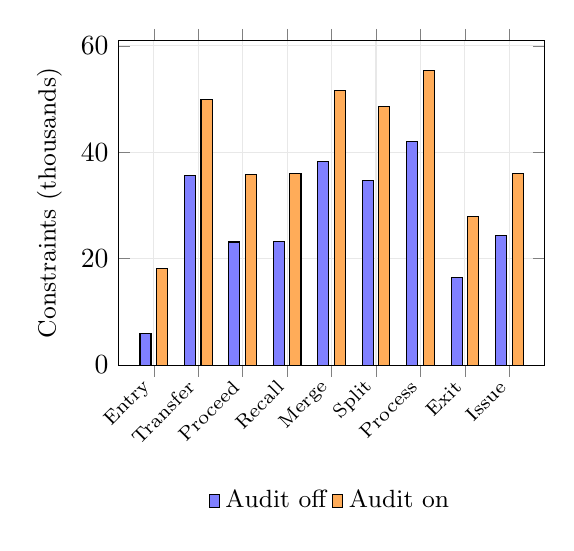
\begin{tikzpicture}\begin{axis}[width=7cm,height=5.7cm,ybar,bar width=4pt,ymin=0,grid=major,major grid style={gray!18},symbolic x coords={Entry,Transfer,Proceed,Recall,Merge,Split,Process,Exit,Issue},xtick=data,x tick label style={rotate=45,anchor=east,font=\scriptsize},ylabel={Constraints (thousands)},label style={font=\small},legend style={at={(0.5,-0.35)},anchor=north,legend columns=2,draw=none,font=\small},legend image code/.code={\draw[#1] (0cm,-0.08cm) rectangle (0.13cm,0.08cm);} ]
            \addplot[fill=blue!50] coordinates {(Entry,5.98) (Transfer,35.645) (Proceed,23.123) (Recall,23.252) (Merge,38.208) (Split,34.671) (Process,42.067) (Exit,16.407) (Issue,24.424)};
            \addplot[fill=orange!65] coordinates {(Entry,18.115) (Transfer,49.883) (Proceed,35.858) (Recall,35.987) (Merge,51.543) (Split,48.608) (Process,55.402) (Exit,27.94) (Issue,35.957)};
            \legend{Audit off,Audit on}\end{axis}\end{tikzpicture}\hspace{0.25cm}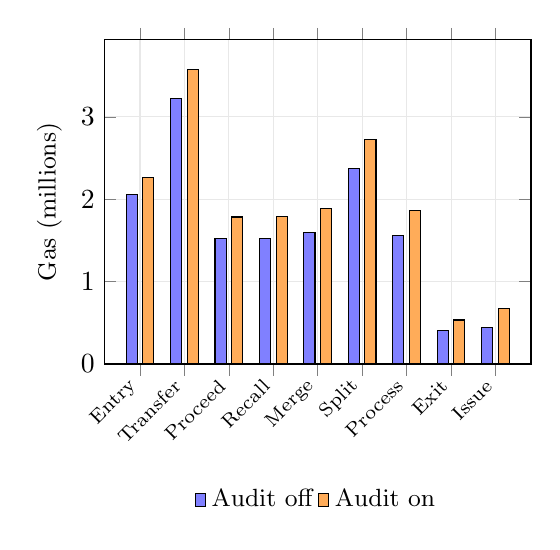
\begin{tikzpicture}\begin{axis}[width=7cm,height=5.7cm,ybar,bar width=4pt,ymin=0,grid=major,major grid style={gray!18},symbolic x coords={Entry,Transfer,Proceed,Recall,Merge,Split,Process,Exit,Issue},xtick=data,x tick label style={rotate=45,anchor=east,font=\scriptsize},ylabel={Gas (millions)},label style={font=\small},legend style={at={(0.5,-0.35)},anchor=north,legend columns=2,draw=none,font=\small},legend image code/.code={\draw[#1] (0cm,-0.08cm) rectangle (0.13cm,0.08cm);} ]
            \addplot[fill=blue!50] coordinates {(Entry,2.059123) (Transfer,3.221268) (Proceed,1.519228) (Recall,1.520722) (Merge,1.599289) (Split,2.373759) (Process,1.557348) (Exit,0.403572) (Issue,0.438706)};
            \addplot[fill=orange!65] coordinates {(Entry,2.258715) (Transfer,3.577414) (Proceed,1.784082) (Recall,1.785084) (Merge,1.888301) (Split,2.730046) (Process,1.866617) (Exit,0.534277) (Issue,0.678565)};
            \legend{Audit off,Audit on}\end{axis}\end{tikzpicture}\end{center}
{\small 그림 1. Event별 Audit 추가 비용. 두 패널의 단위가 다르다.}\par
\begin{center}\small\setlength{\tabcolsep}{6pt}
    \textbf{표 4. Audit 유무와 증가량}\par\smallskip
    \begin{tabular}{@{}lrrrrrr@{}}\toprule
        \textbf{Event} & \textbf{$C_{off}$} & \textbf{$C_{on}$} & \textbf{$\Delta C$} & \textbf{$G_{off}$} & \textbf{$G_{on}$} & \textbf{$\Delta G$} \\ \midrule
        Entry          & 5,980              & 18,115            & 12,135              & 2,059,123          & 2,258,715         & 199,592             \\
        Transfer       & 35,645             & 49,883            & 14,238              & 3,221,268          & 3,577,414         & 356,146             \\
        Proceed        & 23,123             & 35,858            & 12,735              & 1,519,228          & 1,784,082         & 264,854             \\
        Recall         & 23,252             & 35,987            & 12,735              & 1,520,722          & 1,785,084         & 264,362             \\
        Merge          & 38,208             & 51,543            & 13,335              & 1,599,289          & 1,888,301         & 289,012             \\
        Split          & 34,671             & 48,608            & 13,937              & 2,373,759          & 2,730,046         & 356,287             \\
        Process        & 42,067             & 55,402            & 13,335              & 1,557,348          & 1,866,617         & 309,269             \\
        Exit           & 16,407             & 27,940            & 11,533              & 403,572            & 534,277           & 130,705             \\
        Issue          & 24,424             & 35,957            & 11,533              & 438,706            & 678,565           & 239,859             \\
        \bottomrule\end{tabular}\end{center}

추가 Constraints는 11,533--14,238개, 추가 Gas는 130,705--356,287이다.
증가율은 각각 31.70--202.93\%, 9.69--54.67\%다.
기본 비용이 작은 Event는 같은 절대 증가량에도 상대 증가율이 커진다.

암호화 관계와 출력 소비값 계산, 추가 public input·calldata 처리, 감사·연결 자료 저장이 이 차이에 포함된다.
따라서 Audit on/off의 Gas 차이는 순수 SSTORE 차이가 아니다.
별도 Transfer 진단의 AuditRecord 조회·저장 294,700 Gas 역시 전체 추가 비용 356,146 Gas와 같은 항목이 아니다.
    {\small 근거: 실험 1·3의 원자료와 기존 비교표 [D1], Transfer 진단 [D7].}\par
